\chapter{Getting started}

\section{Prerequisites}
\label{sec:prerequisites}

  The programs provided by this project build a knowledge graph.  However,
  a knowledge graph store (better known as an RDF store) is not included.

  Through the years various great RDF stores have been developed, including
  \href{https://virtuoso.openlinksw.com/}{Virtuoso},
  \href{https://github.com/4store/4store}{4store} and
  \href{https://www.blazegraph.com/}{BlazeGraph}.  We recommend using one of
  the mentioned RDF stores with the programs from this project.

  Before we can use the programs provided by this project, we need to build
  them.  The build system needs
  \href{https://www.gnu.org/software/autoconf}{GNU Autoconf},
  \href{https://www.gnu.org/software/automake}{GNU Automake},
  \href{https://www.gnu.org/software/make}{GNU Make} and
  \href{https://www.freedesktop.org/wiki/Software/pkg-config/}{pkg-config}.
  Additionally, for building the documentation, a working \LaTeX{} distribution is
  required including the \texttt{pdflatex} program.  Because \LaTeX{} distributions
  are rather large, this is dependency is optional, at the cost of not being able
  to (re)generate the documentation.

  Each component in the repository has its own dependencies.  Table
  \ref{table:dependencies} provides an overview for each tool.  A $\bullet{}$
  indicates that the program (row) depends on the program or library (column).

  Care was taken to pick dependencies that are widely available on GNU/Linux
  systems.

  \hypersetup{urlcolor=black}
  \begin{table}[H]
    \begin{tabularx}{\textwidth}{X *{9}{!{\color{white}\VRule[1pt]}l}}
      \headrow \cellcolor{White}
      & \rotatebox[origin=l]{90}{\href{https://gcc.gnu.org/}{C compiler}\space\space\space}
      & \rotatebox[origin=l]{90}{\href{https://www.gnupg.org/related_software/libgcrypt/}{libgcrypt}}
      & \rotatebox[origin=l]{90}{\href{http://www.librdf.org/}{raptor2}}
      & \rotatebox[origin=l]{90}{\href{http://www.xmlsoft.org/}{libxml2}}
      & \rotatebox[origin=l]{90}{\href{http://www.htslib.org/}{HTSLib}}
      & \rotatebox[origin=l]{90}{\href{https://zlib.net/}{zlib}}
      & \rotatebox[origin=l]{90}{\href{https://www.gnu.org/software/guile}{GNU Guile}}
      & \rotatebox[origin=l]{90}{\href{https://www.gnutls.org/}{GnuTLS}}
      & \rotatebox[origin=l]{90}{\href{https://tug.org/texlive/}{\LaTeX{}}}\\
      \evenrow
      \texttt{vcf2rdf}    & \B & \B & \B &    & \B &    &    &    &\\
      \oddrow
      \texttt{bam2rdf}    & \B & \B & \B &    & \B &    &    &    &\\
      \evenrow
      \texttt{table2rdf}  & \B & \B & \B &    &    & \B &    &    &\\
      \oddrow
      \texttt{json2rdf}   & \B & \B & \B &    &    & \B &    &    &\\
      \evenrow
      \texttt{xml2rdf}    & \B & \B & \B & \B &    & \B &    &    &\\
      \oddrow
      \texttt{folder2rdf} &    &    &    &    &    &    & \B &    &\\
      \evenrow
      \texttt{sg-web}     &    &    &    &    &    &    & \B & \B &\\
      \oddrow
      Documentation       &    &    &    &    &    &    &    &    & \B \\
    \end{tabularx}
    \caption{\small External tools required to build and run the programs this
      project provides.}
    \label{table:dependencies}
  \end{table}
  \hypersetup{urlcolor=LinkGray}

  The manual provides example commands to import RDF using
  \href{https://curl.haxx.se/}{cURL}.

\section{Setting up a build environment}

\subsection{Debian}

  Debian includes all tools, so use this command to install the
  build dependencies:

\begin{siderules}
\begin{verbatim}
apt-get install autoconf automake gcc make pkg-config libgcrypt-dev     \
                zlib-dev guile-2.0 guile-2.0-dev libraptor2-dev texlive \
                curl libxml2-dev
\end{verbatim}
\end{siderules}

\subsection{CentOS}

  CentOS 7 does not include \texttt{htslib}.  All other dependencies can
  be installed using the following command:

\begin{siderules}
\begin{verbatim}
yum install autoconf automake gcc make pkgconfig libgcrypt-devel \
            guile guile-devel raptor2-devel texlive curl libxml2-devel
\end{verbatim}
\end{siderules}

\subsection{GNU Guix}

  If \href{https://www.gnu.org/software/guix}{GNU Guix} is available on your
  system, an environment that contains all external tools required to build
  the programs in this project can be obtained running the following command
  from the project's repository root:

\begin{siderules}
\begin{verbatim}
guix environment -l environment.scm
\end{verbatim}
\end{siderules}

\subsection{MacOS}

  The necessary dependencies to build \texttt{sparqling-genomics} can be
  installed using \href{https://brew.sh/}{homebrew}:

\begin{siderules}
\begin{verbatim}
brew install autoconf automake gcc make pkg-config libgcrypt guile \
             htslib curl raptor libxml2
\end{verbatim}
\end{siderules}

  Due to a missing \LaTeX{} distribution on MacOS, the documentation
  cannot be build.

\section{Obtaining the source code}
\label{sec:obtaining-tarball}

  \begin{sloppypar}
  The source code can be downloaded at the
  \href{https://github.com/UMCUGenetics/sparqling-genomics/releases}%
  {Releases}%
  \footnote{\url{https://github.com/UMCUGenetics/sparqling-genomics/releases}}
  page.  Make sure to download the {\fontfamily{\ttdefault}\selectfont
    sparqling-genomics-\sgversion{}.tar.gz} file.
  \end{sloppypar}

  Or, directly download the tarball using the command-line:
\begin{siderules}
\begin{lstlisting}[language=bash]
curl -LO https://github.com/UMCUGenetics/sparqling-genomics/releases/\
download/(@*\sgversion{}*@)/sparqling-genomics-(@*\sgversion{}*@).tar.gz
\end{lstlisting}
\end{siderules}

  After obtaining the tarball, it can be unpacked using the \texttt{tar}
  command:

\begin{siderules}
\begin{lstlisting}
tar zxvf sparqling-genomics-(@*\sgversion{}*@).tar.gz
\end{lstlisting}
\end{siderules}

\section{Installation instructions}

  After installing the required tools (see section \ref{sec:prerequisites}
  {\color{LinkGray}`\nameref{sec:prerequisites}'}), and obtaining the source
  code (see section \ref{sec:obtaining-tarball} {\color{LinkGray}
    `\nameref{sec:obtaining-tarball}'}), building involves running the following
  commands:

\begin{siderules}
\begin{lstlisting}
cd sparqling-genomics-(@*\sgversion{}*@)
autoreconf -vif # Only needed if the "./configure" step does not work.
./configure
make
make install
\end{lstlisting}
\end{siderules}

  To run the \texttt{make install} command, super user privileges may be
  required.  This step can be ignored, but will keep the tools in the project's
  directory.  So in that case, invoking \texttt{vcf2rdf} must be done using
  \texttt{tools/vcf2rdf/vcf2rdf} when inside the project's root directory,
  instead of ``just'' \texttt{vcf2rdf}.

  Alternatively, the individual components can be built by replacing
  \texttt{make} with the more specific \texttt{make -C <component-directory>}.
  So, to \emph{only} build \texttt{vcf2rdf}, the following command could be
  used:

\begin{siderules}
\begin{verbatim}
make -C tools/vcf2rdf
\end{verbatim}
\end{siderules}

\section{Using a pre-built Docker image}

  A pre-built Docker container can be obtained from the release page.  It
  can be imported into docker using the following commands:

\begin{siderules}
\begin{lstlisting}
curl -LO https://github.com/UMCUGenetics/sparqling-genomics/releases/\
download/(@*\sgversion{}*@)/sparqling-genomics-(@*\sgversion{}*@)-docker.tar.gz
docker load < sparqling-genomics-(@*\sgversion{}*@)-docker.tar.gz
\end{lstlisting}
\end{siderules}

  The container contains both SPARQLing genomics and Virtuoso (open source
  edition).

\chapter{The knowledge graph}

  In this manual we define a \emph{knowledge graph} as a collection of
  facts stated in a coherent way so that inferences can be drawn from
  the explicitly stated facts.  We implement a knowledge graph using the
  Resource Description Framework \citep{Lassila:99:RDF}, hereafter referred
  to as RDF.  The knowledge graph is the main value obtained from this
  project.

  The programs from chapter \ref{chap:command-line}
  {\color{LinkGray}`\nameref{chap:command-line}'} read data in a
  domain-specific format, and translate it into \emph{facts} in the form
  \emph{subject} $\rightarrow$ \emph{predicate} $\rightarrow$
  \emph{object}, which is the form of an RDF triplet.

  Once all desired data is described as RDF triplets, we can use the SPARQL
  Protocol and RDF Query Language \citep{sparql-11}, better known as simply
  ``SPARQL'', to extract knowledge from the facts.

  Stating facts as RDF is a necessary first step to a more powerful inference
  system.  To understand the knowledge graph and its intended use, we can
  think of the knowledge graph as having multiple layers.  Figure
  \ref{fig:layered-knowledge} displays a small example of two layers.

  \begin{figure}[h]
    \begin{center}
    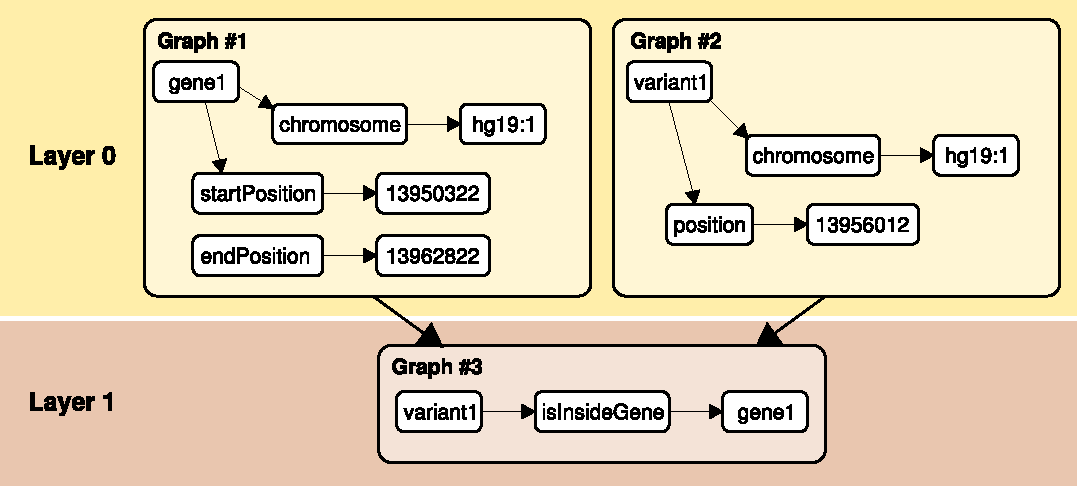
\includegraphics[width=0.9\textwidth]{figures/layered-knowledge.pdf}
    \end{center}
    \caption{\textit{Illustrating knowledge layers.  In the figure we have
        knowledge from two separate sources (gene locations and genomic
        variants) from which we can derive new knowledge in an inference
        layer.}}
    \label{fig:layered-knowledge}
  \end{figure}

  Programs can operate on multiple layers of knowledge.  A program operates
  on the first layer (layer 0) when it translates a non-RDF format into RDF.
  These programs (re)state observations.  In the second layer (layer 1) and
  up, we find programs that operate on facts from layer 0 and generate
  inferences.

  From a computational perspective, these inferences allow programs to take
  shortcuts, and therefore answer questions (called \emph{querying}) faster.
  The performance of querying the graph can therefore be tuned by cleverly
  stating facts.  For example, by using the inference drawn in figure
  \ref{fig:layered-knowledge}, a query asking for ``all variants in a gene''
  no longer needs to compute whether a variant is inside any of the
  genes.  The query planner can also narrow the search space by only
  considering the variants in the layer 1 graph.

  From a data access perspective, these inferences allow fine-grained access
  to knowledge.  For example, access to a layer 1 graph can be given, but
  not to its underlying layer 0 graph(s).  Properties can be removed (like
  patient identifiers), or made less precise (rounding variant positions to
  the nearest 1000).

  \begin{sloppypar}
  The knowledge graph contains two types of nodes; uniquely identifiable
  names having a symbolic value (1), and literal values like numbers and
  text (2).  The symbolic values are written as URIs, for which all symbols
  defined by programs that are part of SPARQLing genomics share a common
  prefix: \texttt{<http://sparqling-genomics/>}.  When we describe a node
  in the remainder of the manual, we shorten the URI with this prefix.
  For example, to describe the URI
  \texttt{<http://sparqling-genomics/Origin/1ec192jh5>}, we could equally
  write \texttt{:Origin/1ec192jh5}, where the colon means ``use the
  common prefix \texttt{<http://sparqling-genomics/>}''.
  \end{sloppypar}

  The programs that are part of SPARQLing genomics use a few patterns to
  come up with identifiers.  For example, to link facts to their original
  (non-RDF) source, we use the type \texttt{:Origin}.  When describing the
  originated file of some facts, we use \texttt{:Origin/}%
  \emph{<SHA256 sum of the file>}, so that we can be sure that when the
  same identifier occurs, the originating bytes are identical.

  In chapter \ref{chap:command-line}
  {\color{LinkGray}`\nameref{chap:command-line}'} we define more types,
  all of them built up from the pattern \texttt{:}\emph{<type name>}%
  \texttt{/}\emph{<string>}.  This can be used as a guideline to interact
  and extend the knowledge graph.

  We attempt to provide the practical tools to build and maintain a flexible
  knowledge graph, and these tools may change over time.  When writing new
  tools or changing existing ones, please consider the effect on the knowledge
  graph first.
